\documentclass[11pt]{article}
\usepackage[margin=1in]{geometry}
\usepackage{graphicx}

\title{\textbf{Key Exchange Outside of TCP / IP}\\ 
{\normalsize Design Document} \\
{\normalsize Group: sdmay20-52}}
\author{Client/Faculty Advisor: Julie Rursch\\
\\
		Jacob Moody\\
		Jack Potter\\
		Andre Chickering\\
		Jordan Svoboda\\
		Joel Wacker\\
		Logan Woolery
}
\date{December 8th, 2019}
\textit{Revised April 20th, 2020}
\begin{document}

\maketitle
\newpage
% The asterisks are necessary to keep these from being counted in ToC
\section*{Executive Summary}

In brief, our project aims to provide a secure means of exchanging keys in a zero trust environment, enabling the foundations for absolute security in communications. In order to facilitate this, we aim to provide a user friendly client capable of exchanging keys in a scenario where no part of the internet is considered safe, and exchange data in an environment where each node in the route could be completely compromised, all while keeping the data confidential.

\subsection*{Engineering Standards and Design Practices}
Our project does not require any circuit or hardware design, so all we will be focusing our efforts on good software practices. Some of the specific practices will be the use of a Git repository to store our code, testing early and testing often, consistent styling and quality comments in our code. \\

We will use a Git repository to store our code and for version control. Git allows us to make branches for testing new changes without breaking any of the working code that we already have and branches also allow us to easily track changes that have been made to our project so we can monitor the progress being made. Another benefit to using Git is that it keeps all of the code from our project centralized for all developers. This centralization makes it extremely easy for all users to get access to the most up to date code, preventing us from wasting time sharing code and trying to figure out where new code fits into the current code base. An Additional benefit of this centralization is that our code is always remotely backed up, so we can access it from anywhere and limiting the effects that a data loss would have on our development abilities. \\

We also plan to test early and often throughout our project development. Any new features will need to be thoroughly tested individually as well as alongside the already implemented features. This will save us time as the project progresses, since any major bugs will be found and fixed while there is only a small amount of code to look at, as opposed to digging through the entire project at the end of its development hunting for the source of bugs. \\

Consistent styling will keep our code readable and make it easier for all developers to understand. By ensuring that all of our code is formatted in the same way, all developers on our team will only need to spend a minimal amount of  time trying  to understand code they didn’t write and they won’t have to decipher another members style choices, allowing them to focus only on what the code does and how it interacts with new code that is being developed. \\

Quality commenting will also contribute to minimizing the amount of time each member spends trying to understand code being written by other members. Our functions should be written in a way that makes them easy to read and understand without comments, but as with any project this is easier said than done. Any code that is written will need to have quality comments that summarize the functionality of that piece of code. These comments will allow developers to spend less time trying to understand code they didn’t write and more time developing the features that interact with that code. \\

We also plan to follow industry standards for information security. One of these is the use of cryptographically secure random number generators to prevent generated keys from being predicted or reverse engineered. Any random numbers used in our application will be generated in part using a source of true randomness, making it near impossible to replicate the values that are being generated. We will also implement encrypted storage of data on our servers to prevent them from being compromised by malicious users. Even if an unauthorized user gained access to our server they would only be presented with a mess of encrypted data that would not disclose any information that is on the servers.


\subsection*{Summary of Requirements}
This project has fairly minimal hardware and software requirements necessary to produce our final product. The hardware requirements for this project consist of computers on which we will perform development work, a server that will host the backend infrastructure for our project, and several cell phones on which the application we develop can be deployed for testing purposes. The software requirements for the development of our project can be broken down into the integrated development environments (IDEs) necessary to build and deploy our application as well as the infrastructure software required for deploying and testing our backend code including a hypervisor and firewall. \\ 

The computers necessary for the development of our project will primarily consist of our own personal laptops and desktops, which will be largely be sufficient. However, we have found the need to source an additional Apple laptop/desktop of any kind, as there are numerous issues preventing the development of iOS applications on anything other than a computer running macOS. The server hardware necessary for hosting our project’s backend will also likely consist of our own server(s). While we initially approached the university to request a virtual private server or a world-routable IP address that could forward traffic to a server we would provide, we encountered difficulties that rendered pursuing the issue untenable. Instead, we will simply use our own servers which already have hypervisors installed that will make the deployment of a new virtual server very straightforward. Finally, between the members of the group, we have a selection of various iPhone and Android cell phones, which will allow testing across numerous platforms.  \\

All of the software required for the development of this project is free and/or open source, eliminating software costs as a constraint on our project. The Android Studio and XCode IDEs will be used for the development and deployment of the phone applications, and team members will be free to utilize their own editors and workflows for the rest of the project.

\subsection*{Applicable Courses from ISU Curriculum}
We will draw from our experiences in the following courses throughout the completion of this project:\\
\begin{itemize}
	\item{Computer Science 309}
	\begin{itemize}
		\item{Software development best practices}
		\begin{itemize}
			\item{Version control using Git}
			\item{Continuous integration using Git/Jenkins}
			\item{Test driven development with unit testing}
		\end{itemize}
		\item{Android application development}
		\begin{itemize}
			\item{Use of Android Studio IDE}
			\item{Integration of external Java libraries}
		\end{itemize}
		\item{Client/server communications}
		\begin{itemize}
			\item{Restful APIs}
			\item{WebSockets}
			\item{Client login and authentication}
		\end{itemize}
	\end{itemize}
	
	\item{Computer Engineering 308}
	\begin{itemize}
		\item{Low-level coding practices}
		\begin{itemize}
			\item{Multithreaded application development}
			\item{Thread-safe programming}
			\item{Understanding of Unix system calls}
			\item{Network communications at low levels}
		\end{itemize}
	\end{itemize}
	
	\item{Computer Science 228}
	\begin{itemize}
		\item{Data Structures}
		\begin{itemize}
			\item{Storing messages, conversations, users efficiently}
			\item{Ensure messages and conversations can be easily searched}
			\item{Store key hashes efficiently}
		\end{itemize}
		\item{Algorithms}
		\begin{itemize}
			\item{Searching conversations/messages}
			\item{Connecting users for conversations}
			\item{Generating/sharing keys quickly}
		\end{itemize}
	\end{itemize}
	
	\item{Computer Engineering 234X}
	\begin{itemize}
		\item{Ethical Considerations}
		\begin{itemize}
			\item{Ensuring we have no access to user messages/keys}
		\end{itemize}
		\item{Legal Considerations}
		\begin{itemize}
			\item{Exporting cryptography suites internationally}
			\item{Responses to law enforcement requests}
		\end{itemize}
	\end{itemize}
	
	\item{Computer Engineering 430/530}
	\begin{itemize}
		\item{Network protocols and security}
		\begin{itemize}
			\item{Network stacks}
			\item{Protocol weaknesses and securities}
		\end{itemize}
	\end{itemize}
\end{itemize}

\subsection*{New Skills/Knowledge acquired that was not taught in courses}
The two primary technologies that we will use that have not been taught in a class before are Go and Flutter. Go is an extremely versatile language developed by Google that will make up the majority of our backend code. We chose to use Go for several reasons. First of all, it is very extensible and makes it very easy to implement open source libraries for cryptography and secure network communications that have been thoroughly audited to ensure efficient and secure performance. Second, Go makes developing test suites in real time very straightforward, and it contains a number of useful utilities to ensure complete coverage of all code by the test suites. Finally, Go can easily export executable builds of our project that can be run on nearly any architecture or operating system very easily. 
\\
We will be using Flutter for the development of our client applications. Flutter is a Google project that allows mobile applications to be developed once in the Dart language and then built into native executables for both Android and iOS. We chose Flutter as it will ensure that all versions of our client application will feel and work similarly, and while we may need to do some manual tweaking for each platform, it will generally increase the efficiency of our development and ensure all features are consistent across both applications.
\\

\newpage
\tableofcontents
\listoffigures
\listoftables
\newpage

\section{Introduction}
\subsection{Acknowledgement}
We are grateful for the opportunity to work on a project envisioned, researched and designed by our group. As we are not professional engineers yet, it is a gift to be able to work with other students who have a similar desire to learn about and implement a topic that we share a passion for. Thank you to Iowa State University for allowing us to pursue this project and providing us the support necessary to complete the project. Thank you also to Dr. Julie Rursch for her mentorship throughout this process. \\

\subsection{Problem and Project Statement}
In an era dominated by mobile devices and messaging applications, there are many choices for how to communicate with friends, family, or coworkers. These applications all function the same for the most part, and most of them will securely exchange your messages. The messages and the keys used for message exchange can be intercepted at some point during the communication by an attacker carrying out a Man-in-the-Middle (MitM) attack. This would allow the attacker to impersonate a node in the communication, allowing them to receive all messages before forwarding them along to their intended recipient. \\

To fully understand the issues with traditional key exchange, some background on symmetric and  asymmetric (also known as public-key) cryptography is needed. In symmetric cryptography, two users have the same key that is used for both encryption and decryption of messages. Since the same key is used for both encryption and decryption, it is especially important to keep it out of the wrong hands. In asymmetric cryptography, a user has two different keys: a public key and a private key. The public key is to be shared with other people and is used for encryption of messages that are to be sent to the key’s owner. The private key must be kept secret and is used for decryption of messages that were encrypted using the public key. \\

Asymmetric cryptography also allows for the signing of messages to verify that the person sending it is who they say they are. Since a user is the only person who has access to their private key (in theory), by encrypting a message with the private key they can let other users know they are the one who sent the message. The recipients can then use the public key to decrypt this, and they will know that the sender is who they claim to be. \\

Generally, symmetric and asymmetric encryption schemes are used in tandem. Symmetric encryption tends to be faster than asymmetric encryption, so it is used for most of the  encrypting and decrypting of messages. Asymmetric cryptography can be used to exchange the symmetric keys since these tend to be smaller than normal messages and therefore not as resource intensive to encrypt, and the key will be more secure in transit since only the intended recipient of the symmetric key will have the means to decrypt it if asymmetric encryption is used. The encrypted symmetric key can also be signed, so it is easier to verify who it was sent from and whether or not it can be trusted. However, the encrypted symmetric key must still be passed over a network, allowing a malicious user to sniff the network traffic to obtain the encrypted key and potentially decrypt it if the encryption algorithm is weak or if they manage to obtain the key needed to decrypt it. \\

The focus of our project is to provide a practical way to exchange the symmetric key needed for message encryption and decryption without having that key ever touch TCP/IP (Transmission Control Protocol over Internet Protocol), meaning it will not be sent over any networks. More specifically, we will be creating our own messaging application for iOS and Android that is capable of exchanging keys in person only, so that these keys can not be intercepted by an attacker. The goal of such an exchange is to establish a shared secret in preparation for secured communications at distance in the future. This initial key exchange does require all users who wish to communicate to engage in a one-time meeting in person prior to opening communication channels that connect the users. Encryption of messages provides privacy and security for the users, preventing prying eyes from reading sensitive messages. If an attacker were to gain access to any of the keys being transmitted the privacy and security gained by encrypting the messages is lost instantly, so our goal is to minimize the opportunity that attackers have to steal the keys. \\

Our plan, as stated briefly above, is to develop a messaging application for users who wish to have a more secure method of key exchange. It shall provide a framework for communication of cryptographic keys in an atypical form of communication, devoid of interactions with any internet protocol communications. One such implementation will be through the use of QR codes, which can be locally generated, shared, and removed, without risk of leaking the cryptographically sensitive materials or even announcing to a greater audience that such an exchange has occurred. After the symmetric key is jointly generated and shared, it will be used to encrypt and decrypt all messages that are shared as a part of its respective conversation. This key is maintained for as long as the conversation lasts, with users free to meet up at any point to establish additional conversations with different keys and/or migrate to a new conversation entirely. We want to ensure that we, as the developers/maintainers/application owners, don’t have access to anything other than the encrypted message and that we have no way to decrypt the messages that are being sent on the application. This will provide security and peace of mind for our users. It is important to note that our server software will be freely available to users, allowing them to run their own servers that they can independently audit to be secure. 


\subsection{Operational Environment}
Our messaging application is intended to operate on any iOS or Android platform. This means that it could be used in any part of the world or any time of day, so we need to keep it uniform across all devices. The fact that it could be used in any part of the world means that the security of our application must be as strong as possible so that no one (from a single hacker sitting in a coffee shop to a hostile foreign government) is able to crack the encryption and read the messages that are being sent. In relation to time of day, we need to ensure that the application is up and running whenever a user wishes to send or receive a message. \\

\subsection{Requirements}
We have a clearly defined set of requirements and goals for our project, which are explained in detail in Section 3.7. A summary of the requirements is as follows:

\subsubsection*{Functional Requirements}
\begin{enumerate}
	\item{Our project must be cross-platform, with Android and iOS client applications as well as portable server software.}
	\item{Our project must achieve secure symmetric key generation and sharing between clients in close physical proximity without the use of any network technologies.}
	\item{Our project must implement an API for our server software that utilizes RESTful communication between the clients and server for message sending and receiving.}
	\item{Our project must encrypt user messages using secure symmetric cryptography and then route those messages between users by utilizing public key cryptography for verifying message integrity and destination.}
\end{enumerate}

Our first functional requirement is that we will have both an Android and iOS application for our messaging application. This way the largest possible amount of users can access and use our application, increasing the impact it will have. Our server also must be portable to numerous operating systems.\\

Our second requirement is to perform no key exchange over TCP/IP. When the key exchange is performed using this protocol, it is susceptible to being observed or intercepted by a malicious party. Our application is seeking to avoid this. The keys will be collaboratively generated by two clients that communicate via a visual medium that cannot be intercepted by adversarial parties.\\

Our third requirement is to use a RESTful API. This allows for ease of communication between the client and the server by allowing us to levy the well tested and performative HTTP libraries for both Flutter and Go. Included within this is that content transferred over HTTP  is encoded using the JavaScript Object Notation(JSON), this allows for a simple marshaling and unmarshaling of data structures across languages. \\

Finally, our fourth requirement is to ensure that cryptographically secure symmetric keys are generated and utilized for message encryption. Following the encryption of a message, it will have the recipient’s public key fingerprint appended to demarcate its designation, and then the entire message is signed with the sender’s public key. This will allow the server to verify message integrity and ensure that messages are routed to the correct users.\\

\subsubsection*{Financial Requirements}
\begin{enumerate}
	\item{We will need a server to host our server software.}
	\item{We will need Android and iOS phones to run the client applications on.}
\end{enumerate}
The first requirement is for a server that we can use to host our application’s web server. This will contain all of the messages (still encrypted, we will NOT be able to read them) as well as handle the transfer of messages between clients. This cost would be estimated to be around \$100 per year if we sought out a virtual private server from a hosting provider, however, we will instead have a group member host the server software on their existing server hardware–  bringing the group’s hosting costs down to \$0. We will also need an Android and an iOS device to test our application on, but this cost shouldn’t be an issue as most people have one of these two devices and our group will have one of each already.

\subsection{Intended Users and Uses}
Our intended users are those that desire an extremely secure yet straightforward way to communicate with each other across networks that are known to be hostile. The use case is somewhat narrowed by the caveat that the users must physically meet in person to generate the encryption keys that will be used for their conversation, however, there are several use cases in which this is an acceptable compromise to ensure strengthened security.\\

One potential use case involves users who are actively protesting a federal government that can intercept internet traffic and potentially launch man-in-the-middle attacks against communications used to establish or share encryption keys.  Protesters would be able to meet in person to generate and exchange encryption keys before using the platform to coordinate direct actions against the government.\\

Another use case would be journalists traveling to a region where their communications will be monitored for espionage purposes. They would be able to coordinate encryption keys before traveling and then utilize the platform to transmit their reporting back to their organization.\\

Finally, a potential group of users for our project are privacy and security advocates. Many individuals who study or work in the security fields use secure communication platforms out of principle, and it’s believable that a large number of them would be interested in utilizing our platform for secure communication.


\subsection{Assumptions and Limitations}
\subsubsection*{Assumptions}
\begin{itemize}
	\item{We will have many simultaneous users interacting with each other through the 	application at any given time.}
	\item{This product will be used on both iOS and Android devices, and these two platforms will be interacting with each other. In other words, iOS users should be able to communicate with Android users and vice versa.}
	\item{Our users will be in close proximity with each other at least once so that they can exchange keys in person.}
	\item{Our application will be used around the world, and not all communications (outside of the initial key exchange) will be occurring at short distances}
\end{itemize}

\subsubsection*{Limitations}
\begin{itemize}
	\item{As this concept has not been implemented in any messaging applications that we know of, we will have to do most of our troubleshooting and testing on our own with little prior art to reference.}
	\item{We will be limited in the number of concurrent users we can have and test with due to the small size of our team and the logistical issues with distributing an application that isn’t on an application store.}
\end{itemize}

\subsection{Expected End Product and Deliverables}
We have developed a plan for the deliverables that we are expecting to complete throughout this project. \\

Our first deliverable that leads to this is a mockup of the application interface for the frontend and the backend server design. For the frontend, we want to make sure we have an idea of what our application should look like. This includes menus, screens, and the functionality that we should be implemented on the client-side. For the backend, we want to have the needed functionality and storage planned out for a prototype of the application to be able to function. This will include the number of messages we want to store, how they will be stored and how they will be delivered. This will ensure we stay on the right track towards a working prototype. Our goal for this deliverable is October 18th, 2019. This date will give us ample time to begin work on a prototype that matches the designs we had.\\

Our ultimate goal is to have a working prototype by the end of the semester. This prototype will be able to exchange keys successfully, but may not have the messaging aspect working completely. This means we will want to have any additional methods of key exchange ironed out and functioning at this time. If we are able to get some messages that can be sent and received, it will be a bonus but we are mainly focused on proving that our concept will work. This will demonstrate that we have a strong foundation going into the second semester and that we will have a working project at the end of our time in senior design. Our date for this deliverable is December 13th, 2019.\\

By the middle of the next semester, we plan to have a working version of the application that is able to exchange keys, send encrypted messages, and decrypt received messages. The goal with this deliverable is to be able to show that we have developed a working application that may still need some polishing but is functional. It should be able to encrypt messages, send them, receive them and decrypt them, as well as exchange the keys in the ways that we implemented in the prototype. This will give us time to make minor improvements and adjustments to the overall application to improve its performance for the user as well as fix any minor issues or bugs that may have arisen. Our date for this deadline is February 10th, 2020.\\

Our final deliverable will be a fully working application that has been optimized and is running as well as we are able to make it. This should have all of the features that we planned implemented and running smoothly, and we will be able to demonstrate that we can communicate with multiple users who all have different keys. There will not be any major bugs/glitches, and the application should be easy to use and efficient. Our date for this deliverable is March 1st, 2020.



\newpage
\section{Specifications and Analysis}
\subsection{Proposed Design}
Our proposed design will be implementing a secure way for keys to be exchanged from peer to peer. To date, we have started implementing a QR code generated key exchange, in which clients will collaboratively generate keys while communicating with QR codes and cameras. We will test this by ensuring that our keys work for clients of different platforms, as well as perform testing of the scalability of our application.\\

    Our functional requirements for our project is cross-platform integration, secure communication, and secure random key generation. To ensure that these functional requirements are secure, we will perform security auditing and testing using common penetration tools, such as Wireshark and Hashcat. Our non-functional requirements will be availability, speed, usability, and overall security while using our application. We will ensure that our application is highly available by offloading some of the verification checks to a centralized server, where the server might cache some of the users’ keys for a period of time. \\
 
    One IEEE standard that would be apply to our project is 802.15.9-2016 which is the IEEE Recommended Practice for the Transport of Key Management Protocol (KMP) Datagrams. This standard focuses on establishing a framework for transporting keys using the Key Management Protocol. This would give engineers a guideline on how to use KMP and would aim to reduce issues that stem from improperly implementing KMP in a product. Our project will be transporting our client’s keys over the air (not using TCP/IP), but we will still need to find a way to securely relay keys over the protocol we use without accidentally exposing sensitive client information.


\subsection{Design Analysis}
Currently, we are developing a client program that will run on Android and iOS. The clients will be exchanging keys using QR codes and the phone’s cameras. Once the keys have been shared between the clients, they will be able to select the server they would like to communicate over. From here, all encryption will be done using AES and the shared key from the QR code. Other methods of key sharing, features, or implementation will probably change as we continue development, but at the current moment, this is the direction that development will be following.\\

The client application is currently a Flutter application that will allow us to easily develop for both iOS and Android. At the moment, we have the Android development environment working. With USB debugging enabled on Android phones, we can run the code and test on actual hardware. iOS, on the other hand, has a higher barrier to development. iOS requires an Apple device (Macbook or otherwise) to test non-Apple store applications on an iPhone. We have not been able to run our application on iOS yet because of the configuration needed between an Apple computer and iPhone.\\

Our Android development is in the beginning stages of implementation. At this moment, we are working on server communications, and have the start of a QR code reader implemented. QR codes have several versions that can be used, from version 1 to 40. Version 40 is the version we will be working with, as it is the most current version, and allows for the greatest amount of encoded data. Our current QR code reader does not seem to support version 40 of QR codes. Reading small QR codes (one that contains short snippets of text, like a URL link) is working as expected. Reading large QR codes currently is resulting in unexpected results. We believe this to be because our current QR code reader does not support version 40 QR codes, and is not able to read codes correctly.\\

One weakness of QR codes is the maximum characters supported. QR codes were not designed for large amounts of text, and are limited to around 4000 characters. As encryption standards continue in their trends of increasing the bits used in keys, QR codes will no longer be able to support their size. Because of this, we are looking at other data sharing options to use. Options could include Bluetooth, audio, or other imagery based sharing.\\

For the server application, we are making use of Communicating Sequential Processes(CSP) design in order to levy Go’s concurrent features. This should allow the server to reply promptly and safely accept and deal with multiple clients. This allows the crucial data structures to be safely guarded within the scope of their concurrent runner, removing the possibility of introducing race conditions by their access.

\subsection{Development Process}
We will be developing our project following the Agile (Kanban “flavor”) process. Developing features quickly and releasing version updates frequently will work best for our type of project as we will be continuously increasing security. We will need to design many parts of the project in parallel, and Kanban’s process will enable us to dive right into producing our product without getting caught up in scheduling weekly meetings or standups outside of our team meetings.


\subsection{Design Plan}
Our project is designed so that our clients can communicate with each other without having to worry about malicious eavesdroppers that would want to prevent or intercept our users’ communications. Potential future users may be whistleblowers trying to spread the word about issues or injustices and may be at risk if communications are intercepted. Journalists in hostile situations, like the protests currently happening in Hong Kong, trying to inform the outside world of what is going on when the people in power are doing everything possible to stop that information from spreading would also find such a tool useful. \\

To achieve this, we will implement client/server communication that will exchange keys using methods other than the TCP/IP protocol. This will increase security for our users as their unique cryptographic keys will never be exchanged over the Internet, reducing the risk of the keys getting intercepted by bad actors. \\

Our clients will be using the Android and iOS mobile platforms, so we will create our frontend for these two platforms. The users will get together and generate a shared symmetric key, as well as share their public keys. The symmetric keys will never leave the device, but the public keys will be stored on a backend database to allow message routing. Note that it is the symmetric key generated on the clients that perform the actual message encryption and decryption. The public keys are used in verification of identity only, as in a web of trust model. \\

Messages that users send from our frontend will be encrypted first using the shared symmetric key and then signed using the recipient’s public key. This methodology provides a multilayered assurance to our end users. The symmetric key encryption is well known to be secure against all forms of attack, while the OpenPGP key uses cryptographic standards well known to be able to verify both the sender of the message as well as guard against undetected modifications of data. \\

Our backend server will only ever see public keys and encrypted message data, but it will have no way to decrypt any of the messages. This database will need to store the encrypted messages that the users exchange, but the messages will still be under strong encryption with no logs stored, and message data will be deleted at user request, all to uphold the users’ expected confidentiality and security while using our product. We will make use of a RESTful API for handling client communications with the server, as this will allow both Android and iOS devices to make requests for stored messages and send new messages to the server for distribution.



\newpage
\section{Statement of Work}
\subsection{Previous Work and Literature}
To our knowledge, this is the first attempt to make key exchanges outside of TCP/IP possible. At the time of writing, the only way to do so would be to write down the key and manually type it into the recipient’s machine. Even the current maximum-paranoia applications using public-key encryption still transfer the keys over TCP/IP. \\

Our wrapper application, a secure messaging application, is not a new concept. The major difference between our application and existing systems, like Signal or WhatsApp, is that we allow users full control of their encryption keys, as well as non-standard means of transferring keys practically. These allow for a greater level of security in the transfer of messages. (“Messages” herein is used in the cryptographic context, referring to any piece of data, not necessarily a textual one.)

\subsection{Technology Considerations}
For our program, we are making use of symmetrical and asymmetrical encryption. For the asymmetrical encryption, we are using RSA. We use the asymmetric keys to act as “addresses” for different users. This allows us to have users prove their ownership of their addresses, without using a password or storing sensitive information on the server. This does force us to store the public keys of users, but we have decided that we will not serve as authority for public keys. This bypasses the use of key signing that openGPG makes heavy use of and ultimately led to a denial of service attack done on their key servers. The public keys will be transmitted over the internet, as we have decided to use them as nothing more than unique “addresses”, and are going to use AES256 for the actual encryption of the message context. This allows for the PGP key pair to be  theoretically compromised, without sacrificing the integrity of the message contents. If the server were to be compromised, the loss would be the set of public keys used by the server, and the relationship between public keys could be leaked. Assuming that the PGP keys used are what one could call “throw-away” keys, then this becomes less of an issue as the public keys would not contain any personally identifiable information.\\



\subsection{Task Decomposition}
The major problem is the sharing of unique cryptographic keys in a zero-trust environment, followed by the use of these keys to secure communications across a network that is known to be hostile. This can be broken into these steps: 
\begin{enumerate}
	\item{\textbf{Generate a secure, cryptographically random symmetric key, with each client drawing from cryptographically secure sources of randomness.} The key generation must be completed before any exchange can occur. We will want to use a cryptographically secure source of randomness to avoid the key generation being predictable or reverse engineered. We will need to make sure that the source of our randomness does not allow malicious users to predict values that are generated, and that they cannot deduce any previously generated keys should a key be compromised. There are libraries with functions that implement this functionality for random number generation, so we will make use of those rather than writing our own methods that may be insecure.}
	
	\item{\textbf{Establish a secure, non-TCP/IP communication channel with recipient device.} We will be passing information directly from one device to the other using QR codes and a camera on the device. The keys being exchanged will be translated into a QR code which can only be scanned in person, as this will avoid the need to transmit the information over a network connection. This channel will be secure from attackers trying to sniff the traffic on a network, but it does bring about other security concerns. For this channel to be truly secure, the users will need to ensure that there isn’t a way for an attacker to view the exchange occurring. If an attacker could see the exchange, they could view the QR code and steal it for use in the future to attempt to gain the key. }
	
	\item{\textbf{Verify the identity of the recipient device.}	Verification of device identity should be a straightforward process. If two users trust each other enough to exchange keys in person, then it will be easy to verify that the recipient device is correct since the communicating devices will be in the same room as the parties performing the exchange.}
	
	\item{\textbf{Perform key exchange.} As the symmetric key that will be used for the conversation is generated collaboratively by the client devices, the key exchange takes place throughout the process of creating the key. The devices are placed with their screens facing each other, so that each device may see the other’s screen using its front-facing camera. As the devices draw on their own cryptographically secure sources of randomness, they collaboratively generate a single symmetric key that will be used for their conversation.}
	
	\item{\textbf{Verify key integrity.} Once the exchange has been completed, it is crucial to verify the keys’ integrity. This step will ensure that usable keys have been exchanged and that no information was lost during the exchange. If a usable key has not been generated, the exchange will need to happen again before the two parties go their separate ways because otherwise, it will not be possible to successfully encrypt and decrypt messages that need to be sent in the future.\\
	
Each of these steps is necessary for the protocol to be viable. Each step depends to some degree on the previous, but each step can be treated as it’s on the functional unit in the program.}
	
\end{enumerate}

\subsection{Possible Risks and Risk Management}
One of our main concerns is in the knowledge we have going into the project. While our group is well versed in the security aspect of our project, we will have to do learning and research on the implementation of our ideas. Since we plan to use Flutter to implement the client application, we will need to become familiar with this language. The documentation for Flutter appears to be detailed and some tutorials can walk new users through the process of starting development and we plan to use these extensively. \\

Another area of concern that is related to Flutter development is building the code for both iOS and Android clients. Android code can be built on Windows and Linux systems, so this shouldn’t be a major issue for our group, but the iOS code can only be built and simulated on systems running macOS. Currently, we plan to develop the code on our Windows and Linux machines, since the main point of using Flutter is the same code for both iOS and Android, and then we will use a MacBook to build and test the code on an iPhone whenever we have major updates. This seems to be the best option at our disposal, but if we find a more efficient way to perform these tasks, we will use that instead.

\subsection{Project Proposed Milestones and Evaluation Criteria}
A few major milestones for our group are the following:
\begin{itemize}
	\item{Working client prototype}
	\item{Successful message encryption}
	\item{Communication between two users}
	\item{Usable beta version of application}
	\item{Group chat fully functional}
	\item{All application functionality implemented}
\end{itemize}

More details of these milestones are as follows:

\begin{itemize}
	\item{\textbf{12/06/2019: Working client prototype}\\
	    For this milestone, we plan to have a partially working version of the mobile application that can perform a key exchange and demonstrate that the exchange has been successful. The app should also be able to communicate with the server, but this communication doesn’t need to be encrypted at this point. This will establish a firm foundation to build from throughout the second semester.}
	\item{\textbf{1/18/2020: Successful message encryption}\\
    For this milestone, we will be successful when we can encrypt a message that is sent to a server, received by a client, and the recipient will be able to decrypt the message without errors. Since we will be able to send unencrypted messages already we will need to encrypt the messages and make sure they can be properly decrypted using the keys that are being exchanged.}
    \item{\textbf{1/25/2020: Communication between two users}\\
    For this milestone, we plan to have the chat functionality fully working for chats between two users. This means that users will be able to send messages back and forth, chat history will be retrievable so users can view the whole conversation and the encrypted conversation will be stored and retrieved from the server whenever new messages are sent.}
    \item{\textbf{2/10/2020: Usable beta version of application}\\
    For this milestone, we want to have a working version of the app with the needed functionality at a basic level. This includes chats with other users, key generation and exchange and encrypted message storage on our servers. The server will also be able to handle multiple connections/requests at the same time. We will be using the time from the previous milestone until this one to make improvements to the app so that it is usable and looks professional, and it will also give us some time to test it as a group to ensure it is performing as expected.}
    \item{\textbf{2/24/2020: Group chat fully functional}\\
    As with all messaging applications, group chat functionality is expected by our users. This will be a little trickier to implement than a chat between two users since we will need to generate and share a key with more than just two users, which is not the traditional idea in a key exchange. We want to ensure that the regular chat is fully functionally before this stage and that it has been tested by other users so that we can have a solid foundation to build the group chat functionality from, so this will be implemented two weeks after we begin some of our beta tests.}
    \item{\textbf{3/1/2020: All application functionality implemented}\\
By March 1st, we will have all of the stated functionality for our app so that we have ample time for users to test it and for our team to make fixes when issues are encountered. This functionality will include the key exchange between users, proper encryption/decryption of messages and full chat functionality for both two user chats and group chats. The app should be mostly finished and any further work will be bug fixes and application improvements based on user feedback.}
\end{itemize}

\subsection{Project Tracking Procedures}
We will utilize the Kanban boards that are built into GitHub to establish and track goals and progress. Andre has been elected to serve as a manager tasked with ensuring that we keep achieving goals at an acceptable pace. He will ensure that our metrics regarding percentages of tasks completed are reported back to Dr. Julie Rursch and that corrective actions are taken if necessary to ensure the prompt realignment of our team with our original goals. 
\subsection{Expected Results and Validation}
Our goal is to have a secure, user-friendly method of exchanging keys in a zero-trust environment, and then having a viable means of communicating with these keys, all with no trust in the internet infrastructure. To confirm that we have met these goals, we will perform extensive security testing of our platform. More details of these tests can be found in Section 5 of this document, which outlines some of the tests necessary to ensure that our project goals have been achieved. These goals can be summarized as follows:
\begin{enumerate}
	\item{First and foremost, we will have functional cell phone applications for both the Android and iOS mobile operating systems. We will also have a very portable server application that can be deployed on a variety of operating systems. The client applications will be designed such that they require a form of authentication such as a passphrase before they can be unlocked, and all data stored on the client devices will be kept encrypted at rest and decrypted on the fly after the user has authenticated themselves.}
	\item{Second, we will have two cell phones with our client application collaboratively generate and share a symmetric encryption key. This will occur with no transmissions over any network, including Wi-Fi, GSM, etc. The key will be generated with cryptographically secure sources of randomness, ensuring that not only can the key never be intercepted, but it can not be recreated by an adversary. This collaborative process will also be when the clients exchange their respective public key information for message signing and validation.}
	\item{Third, one of the client devices will compose a message, encrypt it with the appropriate public key, attach the public key of the second client, sign it with their own private key, and then send it to the specified server.}
	\item{Fourth, the server application will receive the incoming message, verify that it has been signed by any user who has previously uploaded their public key, verify that it is destined for another user who has uploaded their public key, and then attempt to route the message to its intended recipient. Depending on each user’s predetermined settings, the message may be kept or automatically deleted from the server once it has been received by the intended recipient. If the message is kept on the server, it remains in the strongly encrypted state it arrived in.}
	\item{Finally, once the second client has received the message, it will be decrypted once the second user inputs their passphrase to unlock the symmetric key used for decryption.}
\end{enumerate}

At every point in this process, we will be testing to ensure no adversary would be able to intercept or produce a plaintext copy of any message or the keys required to encrypt/decrypt messages being sent by legitimate users. To aid in testing, we will distribute our application to several volunteers to send and receive messages while other volunteers who are experienced network security professionals attempt to intercept communications, reproduce the keys of other users, and generally disrupt the service. 

\newpage
\section{Project Timeline, Estimated Resources, and Challenges}
\subsection{Project Timeline}
\begin{figure}[h!]
  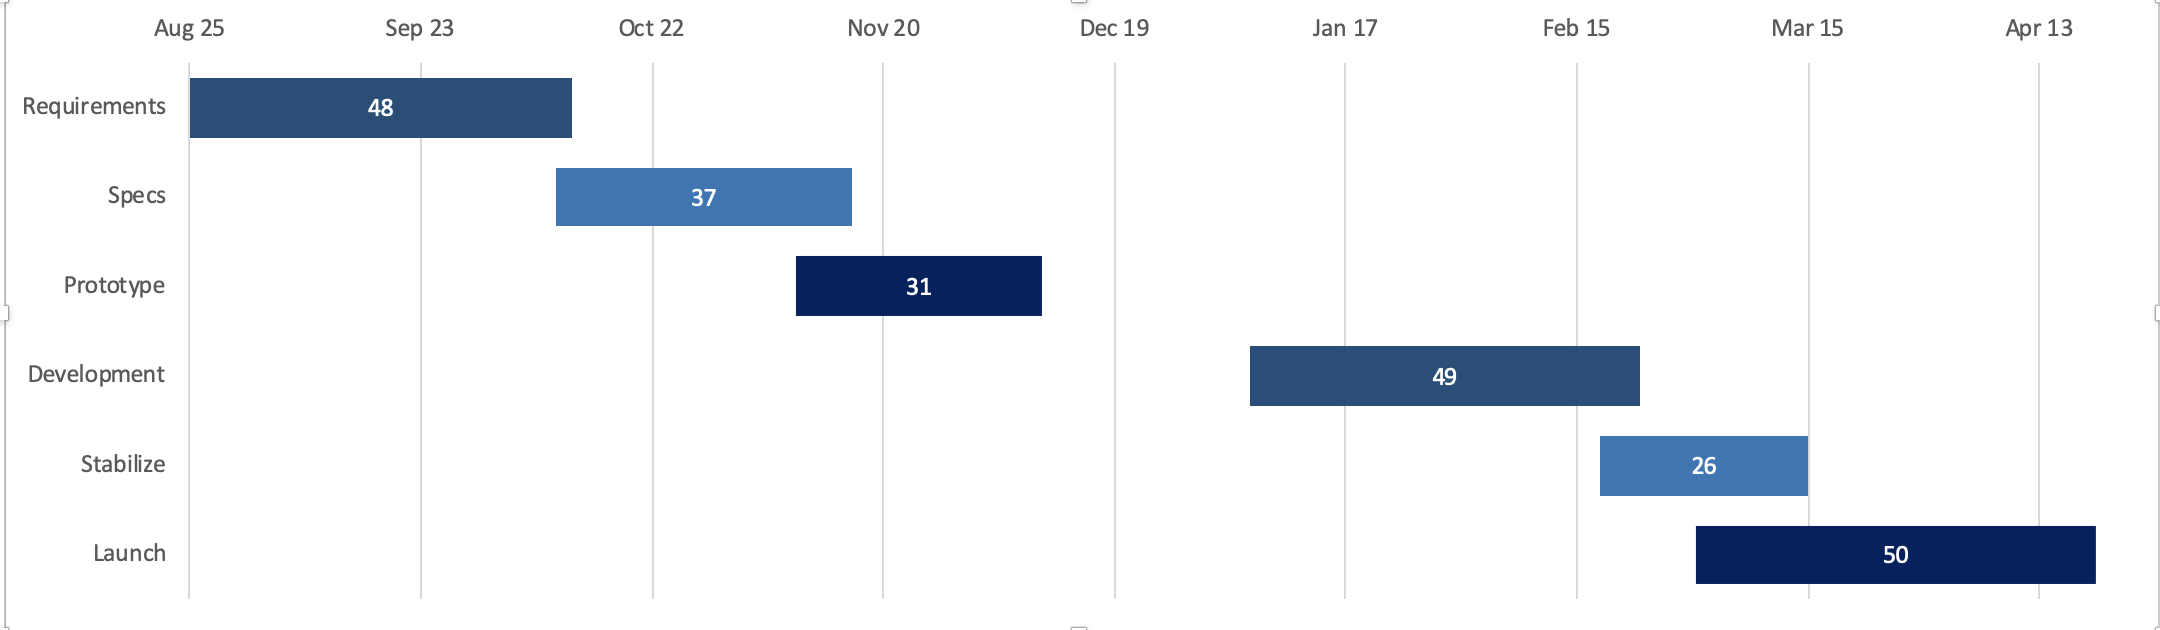
\includegraphics[width=\linewidth]{gantt_chart.png}
  \caption{Project Gantt Chart}
  \label{fig:gantt_chart}
\end{figure}

As illustrated above, we plan to divide the work across the two semesters in a typical fashion. The first semester will be spent largely in Business Analyst style work: developing requirements, setting initial specifications, and heavy client communication. There will also be some initial prototyping work done to help with the finalization of the specifications.

\subsection{Feasibility Assessment}
In our assessments, we have determined this project, as described, to be of appropriate complexity and size for the given time frame. Our major anticipated challenges include cross-platform interoperability, secure non-standard communication, and cross-platform feature parity.

\subsection{Personnel Effort Requirements}
	\begin{table}[h!]
	\begin{center}
		\caption{Task/Time Breakdown}
		\label{tab:table1}
		\begin{tabular}{c|c}
		\textbf{Task} & \textbf{Time} \\
		\hline
		Requirements & 36 Hours \\
		Specifications & 24 Hours \\
		Prototyping & 80 hrs \\
		Development & 180 hrs \\
		Stabilization & 30 hrs \\
		Final Release & 30 hrs \\

		\end{tabular}
	\end{center}
	\end{table}
\subsection{Other Resource Requirements}
This project will require development and testing for our clients and servers. The iOS and Android clients will be tested on an iOS and an Android device respectively, and we have the devices necessary to develop and test our project. We have independently sourced a MacBook to assist in the building and deploying of the iOS client code. \\
\subsection{Financial Requirements}
As this entire project will be developed and completed with free and/or open-source software that will run on hardware that is already owned by our group, we do not anticipate any financial costs at this time. Group members will use their computers to develop the project, and we have a MacBook to assist in building and deploying iOS code. The project will be deployed on server hardware and phones owned by various group members. 

\newpage
\section{Testing and Implementation}

\subsection{Interface Specification}
No special software testing interface will be necessary for the development and deployment of testing suites for our project. The Go programming language testing library will be used to assist in the generation and use of tests of our server infrastructure code. The Flutter testing library will be employed for functional testing of each module in our Android and iOS applications. As no hardware is being developed in this project, we do not need to develop any hardware testing specifications. 

\subsection{Hardware and Software}
Testing for our Flutter application will require us to have Android and iOS devices to place the app on. One of the main features of Flutter development is the “Hot Reload” feature, which allows us to make changes to code and then instantly load the new code and changes to a running device connected to the computer. This will be extremely useful for testing as it will allow us to test the application on real devices, make necessary changes and then test those changes without wasting time compiling new code and moving it around to get it onto devices. This should be the extent of the hardware needed for Flutter testing as other tests will be carried out in software.\\

Flutter also has a testing library built-in, so we will be making use of this. It has built-in unit testing, widget testing, and integration testing with documentation provided for each. The unit tests will be used for testing smaller functions throughout the application, like display values and the logic in the functions. These will be helpful when making smaller changes or when trying to determine the source of bugs. Widget tests are used to test each of the screens in our application and their functionality. These tests will allow us to simulate users interacting with the various screens that we designed and allow us to ensure that button presses result in the correct actions, check that needed elements on the screen are present and test out any other functionality relating to the screens.\\

For the server code, Go offers support for unit testing within the standard library. The Go tests suit supports coverage semantics and offers suggestions for organizing the tests in place with your codebase. For testing the server code we are aiming to have test cases for all success messages and checking to make sure errors are generated expectedly and handled properly. Go’s cross-compilation also allows for tests to be executed for other platforms fairly easy, so it is not difficult to ensure that our server code runs on all of the systems that Go supports.


\subsection{Functional Testing}
\subsubsection*{Unit-Based Testing}
For testing our server-side code, we will create unit tests written in Go, taking advantage of the Go programming language’s built-in testing library. Unit tests will be created incrementally with the server-side code to ensure that our code doesn’t introduce vulnerabilities or bugs that would compromise the security or functionality of our application. To test the iOS and Android clients, we will be using Flutter unit tests.

\subsubsection*{Integration Testing}
Due to the relatively small size of this project, integration testing will come somewhat naturally as we continue to develop both the server and client software. Some automated tests will be used to ensure that client/server communication continues to work throughout development, i.e. ensure that APIs are not modified unexpectedly. Beyond these few tests, further integration tests are not specifically planned at this time, although they may be added if a need becomes obvious. 

\subsubsection*{System Testing}
After our application passes the integration testing phase, we will then ensure that our clients and server communicate and behave as expected. This will include sending malformed requests to ensure the server handles errors properly, verifying that all communications are encrypted and decrypted when appropriate between the clients and the server, and general usability tests.

\subsubsection*{Acceptance Testing}
After our application passes system testing, we are going to have people test our application to make sure that it works. We will attempt to recruit people of all technical skill sets to ensure that our application can be used by everyone. We will be creating documentation of how to create new servers and how to use our application as a whole, and we will also have our users verify that our documentation is articulate, and easy to understand. We will also involve a small group of external users as beta testers once our project is in a feature complete state.

\subsection{Non-Functional Testing}
\subsubsection*{Performance Testing}
Our tests for performance will be performed by the users we distribute the application to. We will need to make sure that users can send messages without a noticeable delay and this test is best accomplished through heavy use by real users. Heavy use by our users will also allow us to test server performance. Since we plan to have users all around the world and have many users at once sending and receiving messages, we will want to perform some “stress tests” to ensure that servers can adequately handle the traffic of multiple users attempting to connect. Periodically we will get feedback from our user base and we will use this to determine where performance is lacking, then refocus our efforts towards fixing these performance issues.

\subsubsection*{Security Testing}
In order to ensure the security of our platform, we will conduct periodic code reviews of our server and client code. We will also conduct at least one penetration test against our service, attempting to circumvent security controls as well as attempt a denial-of-service that leverages a weakness in our platform (distributed denial-of-service is considered outside the scope of our testing). We also intend to invite friends who work as professional penetration testers to launch attacks against our platform to see if they are able to intercept communications or disrupt the service in a preventable way. 

\subsubsection*{Usability Testing}
As soon as our project is in a semi-workable state, we will begin deploying development builds to our server and our personal cell phones. This will give us the opportunity to constantly use the application, finding bugs and noting usability issues in the process. Closer to the end of the development of the project, we will give access to the application to a group of friends and associates who have agreed to test our application and give us feedback on the interface, functionality, and other usability factors. 

\subsubsection*{Compatibility Testing}
As our project is not designed to communicate across platforms other than our own, there are very few points for compatibility issues to arise. We will perform testing with an Android emulator to ensure that our Android application works across a variety of devices, and beyond that, strenuous compatibility testing will not be necessary. Due to the nature of iPhone development, our app will seamlessly work on any iOS phone platform. Our server code can easily be built and run for nearly any operating system on nearly any architecture, thanks to the versatility of the Go programming language, and specifically the power of the "GOOS" environment variable, which allows for effortless cross-compilation.

\subsection{Process}

\begin{figure}[h!]
  \centerline{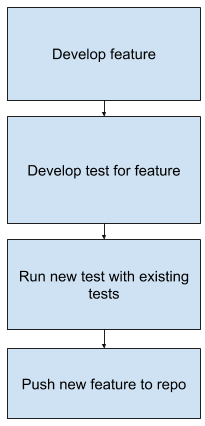
\includegraphics{testFlowchart.png}}
  \caption{Software Test Development Flow Diagram}
  \label{fig:flow_diag}
\end{figure}

For both the client and server program we have multiple continuous integration setup tasks to be run whenever code is pushed or when pull requests are recreated. This has allowed us to quickly recognize whenever issues crop up in either of the code bases.  Ideally tests are run after every feature check by our team, but this has an automated and programmatic way of checking and ensuring this is the case.

\subsection{Results}
Once we started to write some of our server code we realized our original idea of keeping all keys outside of TCP/IP was not exactly what we were looking for. For users to prove their identity, we needed to store the public key of the user on the server and provide proof of their identity by signing their messages. This has led us to add symmetric encryption for the actual message content and use asymmetric encryption only for message signing and for delivering messages to the proper users. This method will still allow us to perform the key exchange outside of TCP/IP, with only the public keys of our users being transmitted across any networks. This was deemed acceptable because we do not serve as the central authority responsible for telling users that a person owns a key. This means that clients do not have to trust our server or the connection from their device to the server to know that their messages are reasonably safe.\\

For our tests, we have been testing with valid RSA keys, for registering users and validating fingerprint ownership. The test data is sent to a local testing server that is spun up when tests start and spun down when they exit. This has allowed us to test JSON marshaling and unmarshalling as well as communication over HTTP.\\

For the clients, we ran into issues with reading very large QR codes (1000 characters or more). With those tools, we have been able to read QR codes containing large public keys on Linux without issue. \\

Currently, we have been able to test key exchange and some server-side functions manually with command-line tools. With the groundwork laid out, we are beginning to develop a mobile client application that will combine all our testing into one package, making our project user-friendly and convenient.

\newpage
\section{Closing Material}
\subsection{Conclusion}

Our focus within the first semester of this project has been on the establishment of languages that we will use, the encryption standards we will use, and deciding how the client and server will pass information back and forth to each other. \\

For the languages, we have focused on Go and Flutter for their high portability and support of features that our application takes advantage of. Both of these languages can be used to develop applications for a multitude of platforms, which will allow our application and ideas to be applied with a much larger reach. \\

For encryption standards we initially chose to use PGP and AES. After beginning client-side development, we determined that PGP did not have the support our application needed, so we switched to using RSA. We expect system admins to use TLS when setting up servers for their own deployments of our application, but it is not required. \\

Our client communicates with the server by making requests to RESTful APIs. These requests are simple JSON objects that contain the information needed by the server to make the request and nothing more. \\

Our goal for next semester is to continue to build on our prototype by fleshing out our user experience, getting feedback and gathering user experience metrics. Our prototype is still fairly basic and going forward we will be adding message encryption and decryption using the keys we generated, creating actual chats to keep track of messages two users have sent to each other and developing a group chat functionality that will allow our to meet the standard users expect from a messaging application.

\subsection{References}
\begin{itemize}
	\item{Jivsov, A. (2012). Elliptic Curve Cryptography (ECC) in OpenPGP. doi: 10.17487/rfc6637}
	\item{Go is an open source programming language that makes it easy to build simple, reliable, and efficient software. (n.d.). Retrieved December 8, 2019, from https://golang.org/.}
	\item{Flutter Documentation. (n.d.). Retrieved December 8, 2019, from https://flutter.dev/docs.}
	\item{National Institute of Standards and Technology (2001). Announcing the ADVANCED ENCRYPTION STANDARD (AES). doi:10.6028/NIST.FIPS.197}
	\item{"802.15.9-2016 - IEEE Recommended Practice for Transport of Key Management Protocol (KMP) Datagrams". IEEE, 17 Aug. 2016, standards.ieee.org/standard/802\_15\_9-2016.html}
\end{itemize}
\subsection{Appendices}
\begin{figure}[h!]
  \centerline{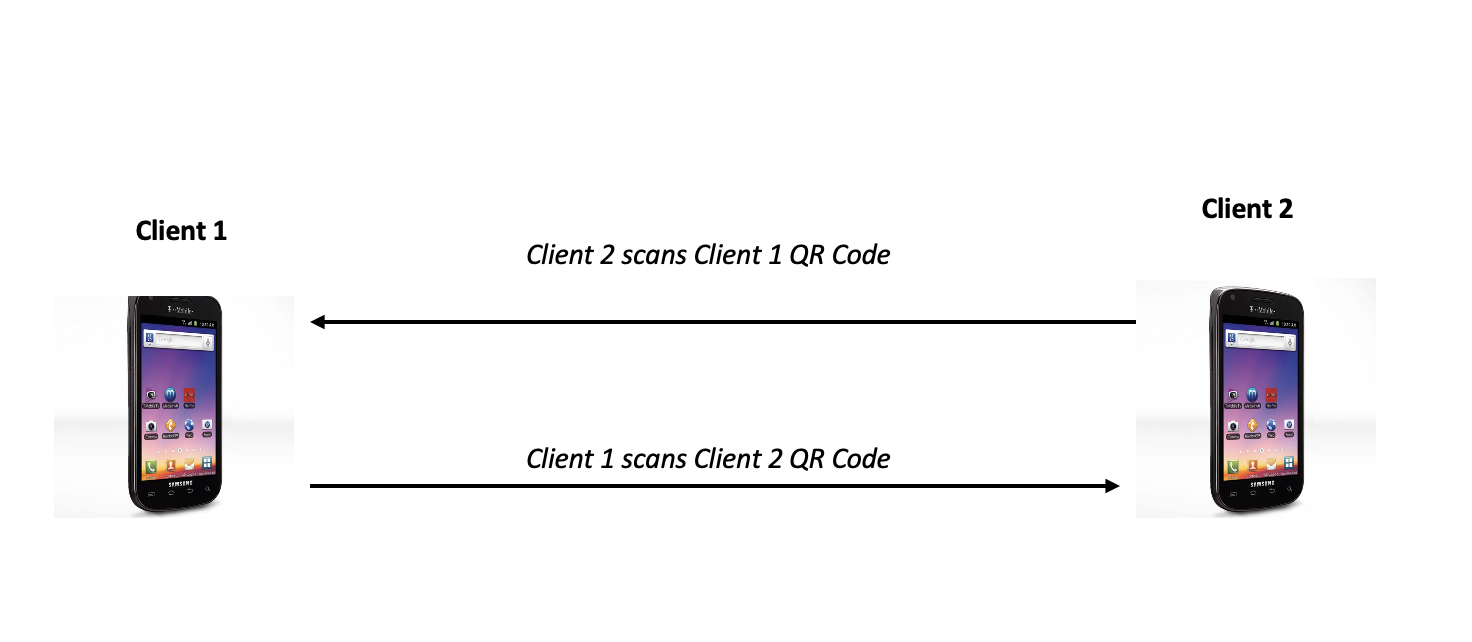
\includegraphics[width=\linewidth]{cc.png}}
  \caption{Client creation and sharing of symmetric keys via QR codes}
  \label{fig:client_client}
\end{figure}

\begin{figure}[h!]
  \centerline{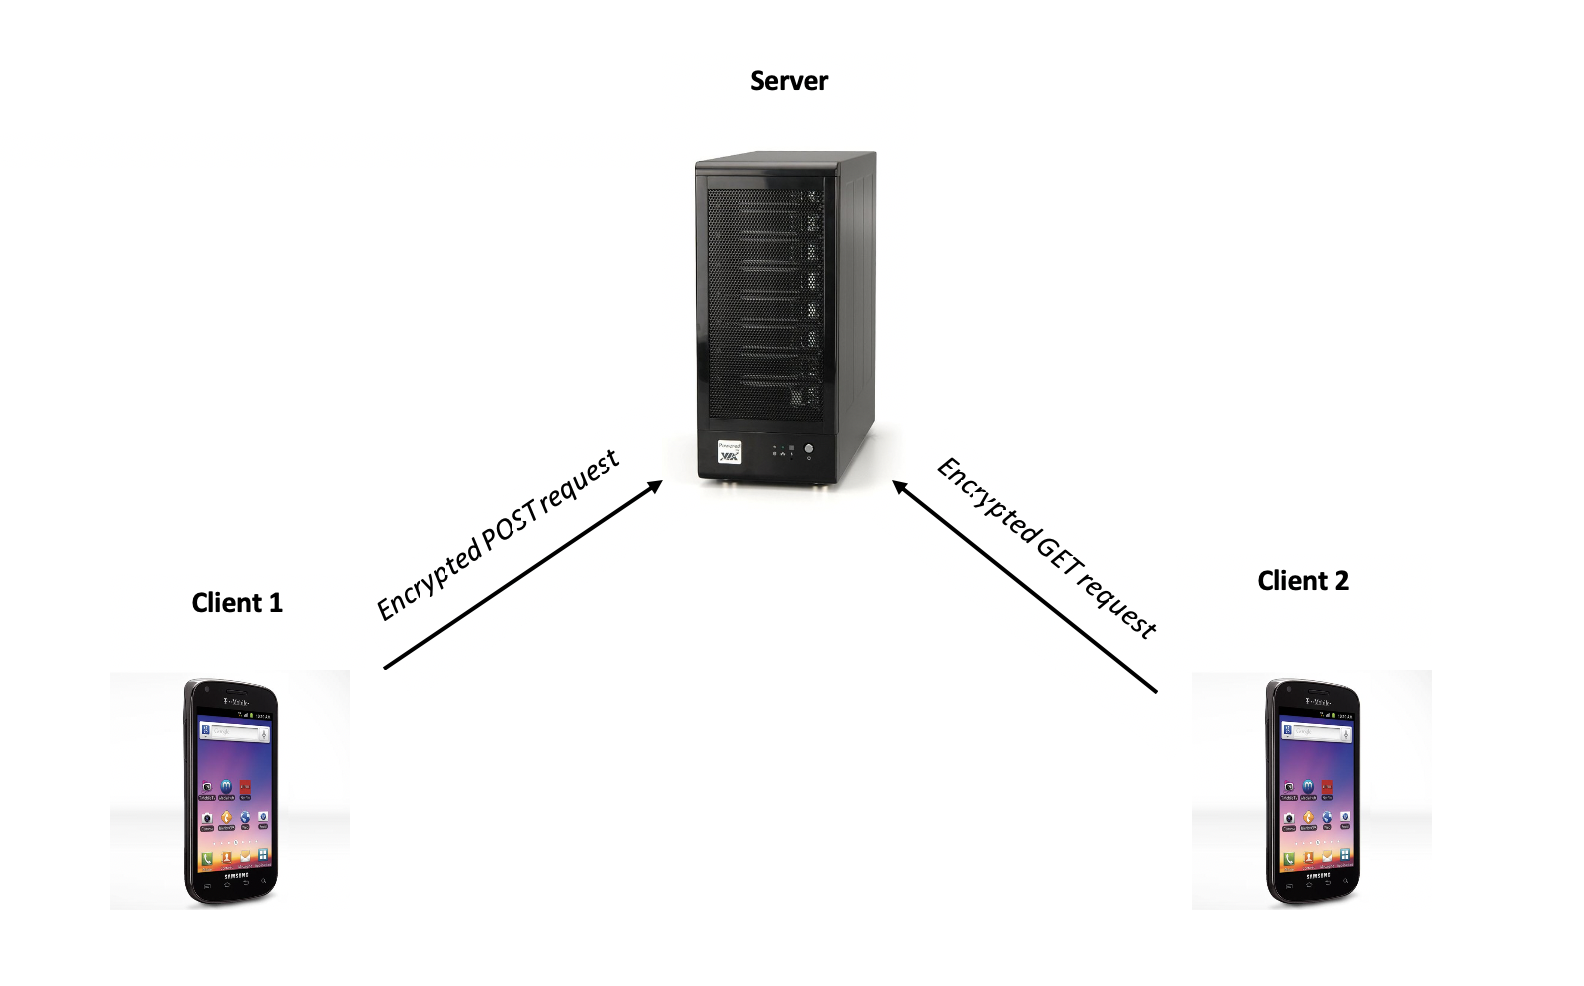
\includegraphics[width=\linewidth]{cs.png}}
  \caption{Communication between clients and server for sending and receiving messages.}
  \label{fig:client_client}
\end{figure}

\end{document}
]